\documentclass[a4paper, 14pt]{extarticle}
\usepackage[russian]{babel}
\usepackage[T1]{fontenc}
\usepackage{fontspec}
\usepackage{indentfirst}
\usepackage{enumitem}
\usepackage{graphicx}
\usepackage[
  left=20mm,
  right=10mm,
  top=20mm,
  bottom=20mm
]{geometry}
\usepackage{parskip}
\usepackage{titlesec}
\usepackage{xurl}
\usepackage{hyperref}
\usepackage{float}
\usepackage[
  figurename=Рисунок,
  labelsep=endash,
]{caption}
\usepackage[outputdir=build, newfloat]{minted}
\usepackage{multirow}
\usepackage{array}

\hypersetup{
  colorlinks=true,
  linkcolor=black,
  filecolor=blue,
  urlcolor=blue,
}

\renewcommand*{\labelitemi}{---}
\setmainfont{Times New Roman}
\setmonofont{JetBrains Mono}[
  SizeFeatures={Size=11},
]

\newenvironment{code}{\captionsetup{type=listing}}{}
\SetupFloatingEnvironment{listing}{name=Листинг}

\setminted{
  fontsize=\footnotesize,
  framesep=0mm,
}

\captionsetup{width=\textwidth,justification=centering}
\captionsetup[table]{singlelinecheck=off,justification=justified}

\newcolumntype{L}[1]{>{\raggedright\let\newline\\\arraybackslash\hspace{0pt}}m{#1}}
\newcolumntype{C}[1]{>{\centering\let\newline\\\arraybackslash\hspace{0pt}}m{#1}}
\newcolumntype{R}[1]{>{\raggedleft\let\newline\\\arraybackslash\hspace{0pt}}m{#1}}

\setlength{\parskip}{6pt}

\setlength{\parindent}{1cm}
\setlist[itemize]{itemsep=0em,topsep=0em,parsep=0em,partopsep=0em,leftmargin=2.0cm}
\setlist[enumerate]{itemsep=0em,topsep=0em,parsep=0em,partopsep=0em,leftmargin=2.0cm}

\renewcommand{\thesection}{\arabic{section}.}
\renewcommand{\thesubsection}{\thesection\arabic{subsection}.}
\renewcommand{\thesubsubsection}{\thesubsection\arabic{subsubsection}.}

\titleformat{\section}{\normalfont\bfseries}{\thesection}{0.5em}{}
\titleformat{\subsection}{\normalfont\bfseries}{\thesubsection}{0.5em}{}

\titleformat*{\section}{\normalfont\bfseries}
\titleformat*{\subsection}{\normalfont\bfseries}

\linespread{1.5}
\renewcommand{\baselinestretch}{1.5}
\begin{document}

\begin{titlepage}
  \vspace{0pt plus2fill}
  \noindent

  \vspace{0pt plus6fill}
  \begin{center}
    Санкт-Петербургский национальный исследовательский университет
    информационных технологий, механики и оптики

    \vspace{0pt plus3fill}

    Факультет инфокоммуникационных технологий

    Направление подготовки 11.03.02

    \vspace{0pt plus2fill}

    Практическая работа №2

    Изучение общих принципов построения IP-сетей \\ (адресация и маршрутизация)

    \vspace{0pt plus1fill}

    Вариант №19

  \end{center}

  \vspace{0pt plus7fill}
  \begin{flushright}
    Выполнил: \\
    Швалов Даниил Андреевич

    Группа: К33211

    Проверил: \\
    Харитонов Антон
  \end{flushright}

  \vspace{0pt plus2fill}
  \begin{center}
    Санкт-Петербург

    2023
  \end{center}
\end{titlepage}

\setcounter{page}{2}

\section{Введение}

\textbf{Цель работы}: изучить основные принципы IP-адресации, получить
практические навыки в построении сетей и подсетей разных классов с
использованием современных возможностей протокола IP, изучить базовые принципы
маршрутизации в IP-сетях, научиться конфигурировать сетевое оборудование с
помощью симулятора CISCO PacketTracer.

\section{Проектирование сети}

\subsection{Структура сети}

В задании моего варианта необходимо использовать маршрутизаторы 1, 3 и 7, а
также сети с номерами 1, 3(5), 5(2), 6(5), где числа в скобках означают
количество подсетей, на которые нужно разбить соответствующие сети. В
соответствии с заданием, структура сети примет вид, изображенный на рис.
\ref{fig:network-scheme-1}.

\begin{figure}[H]
  \centering
  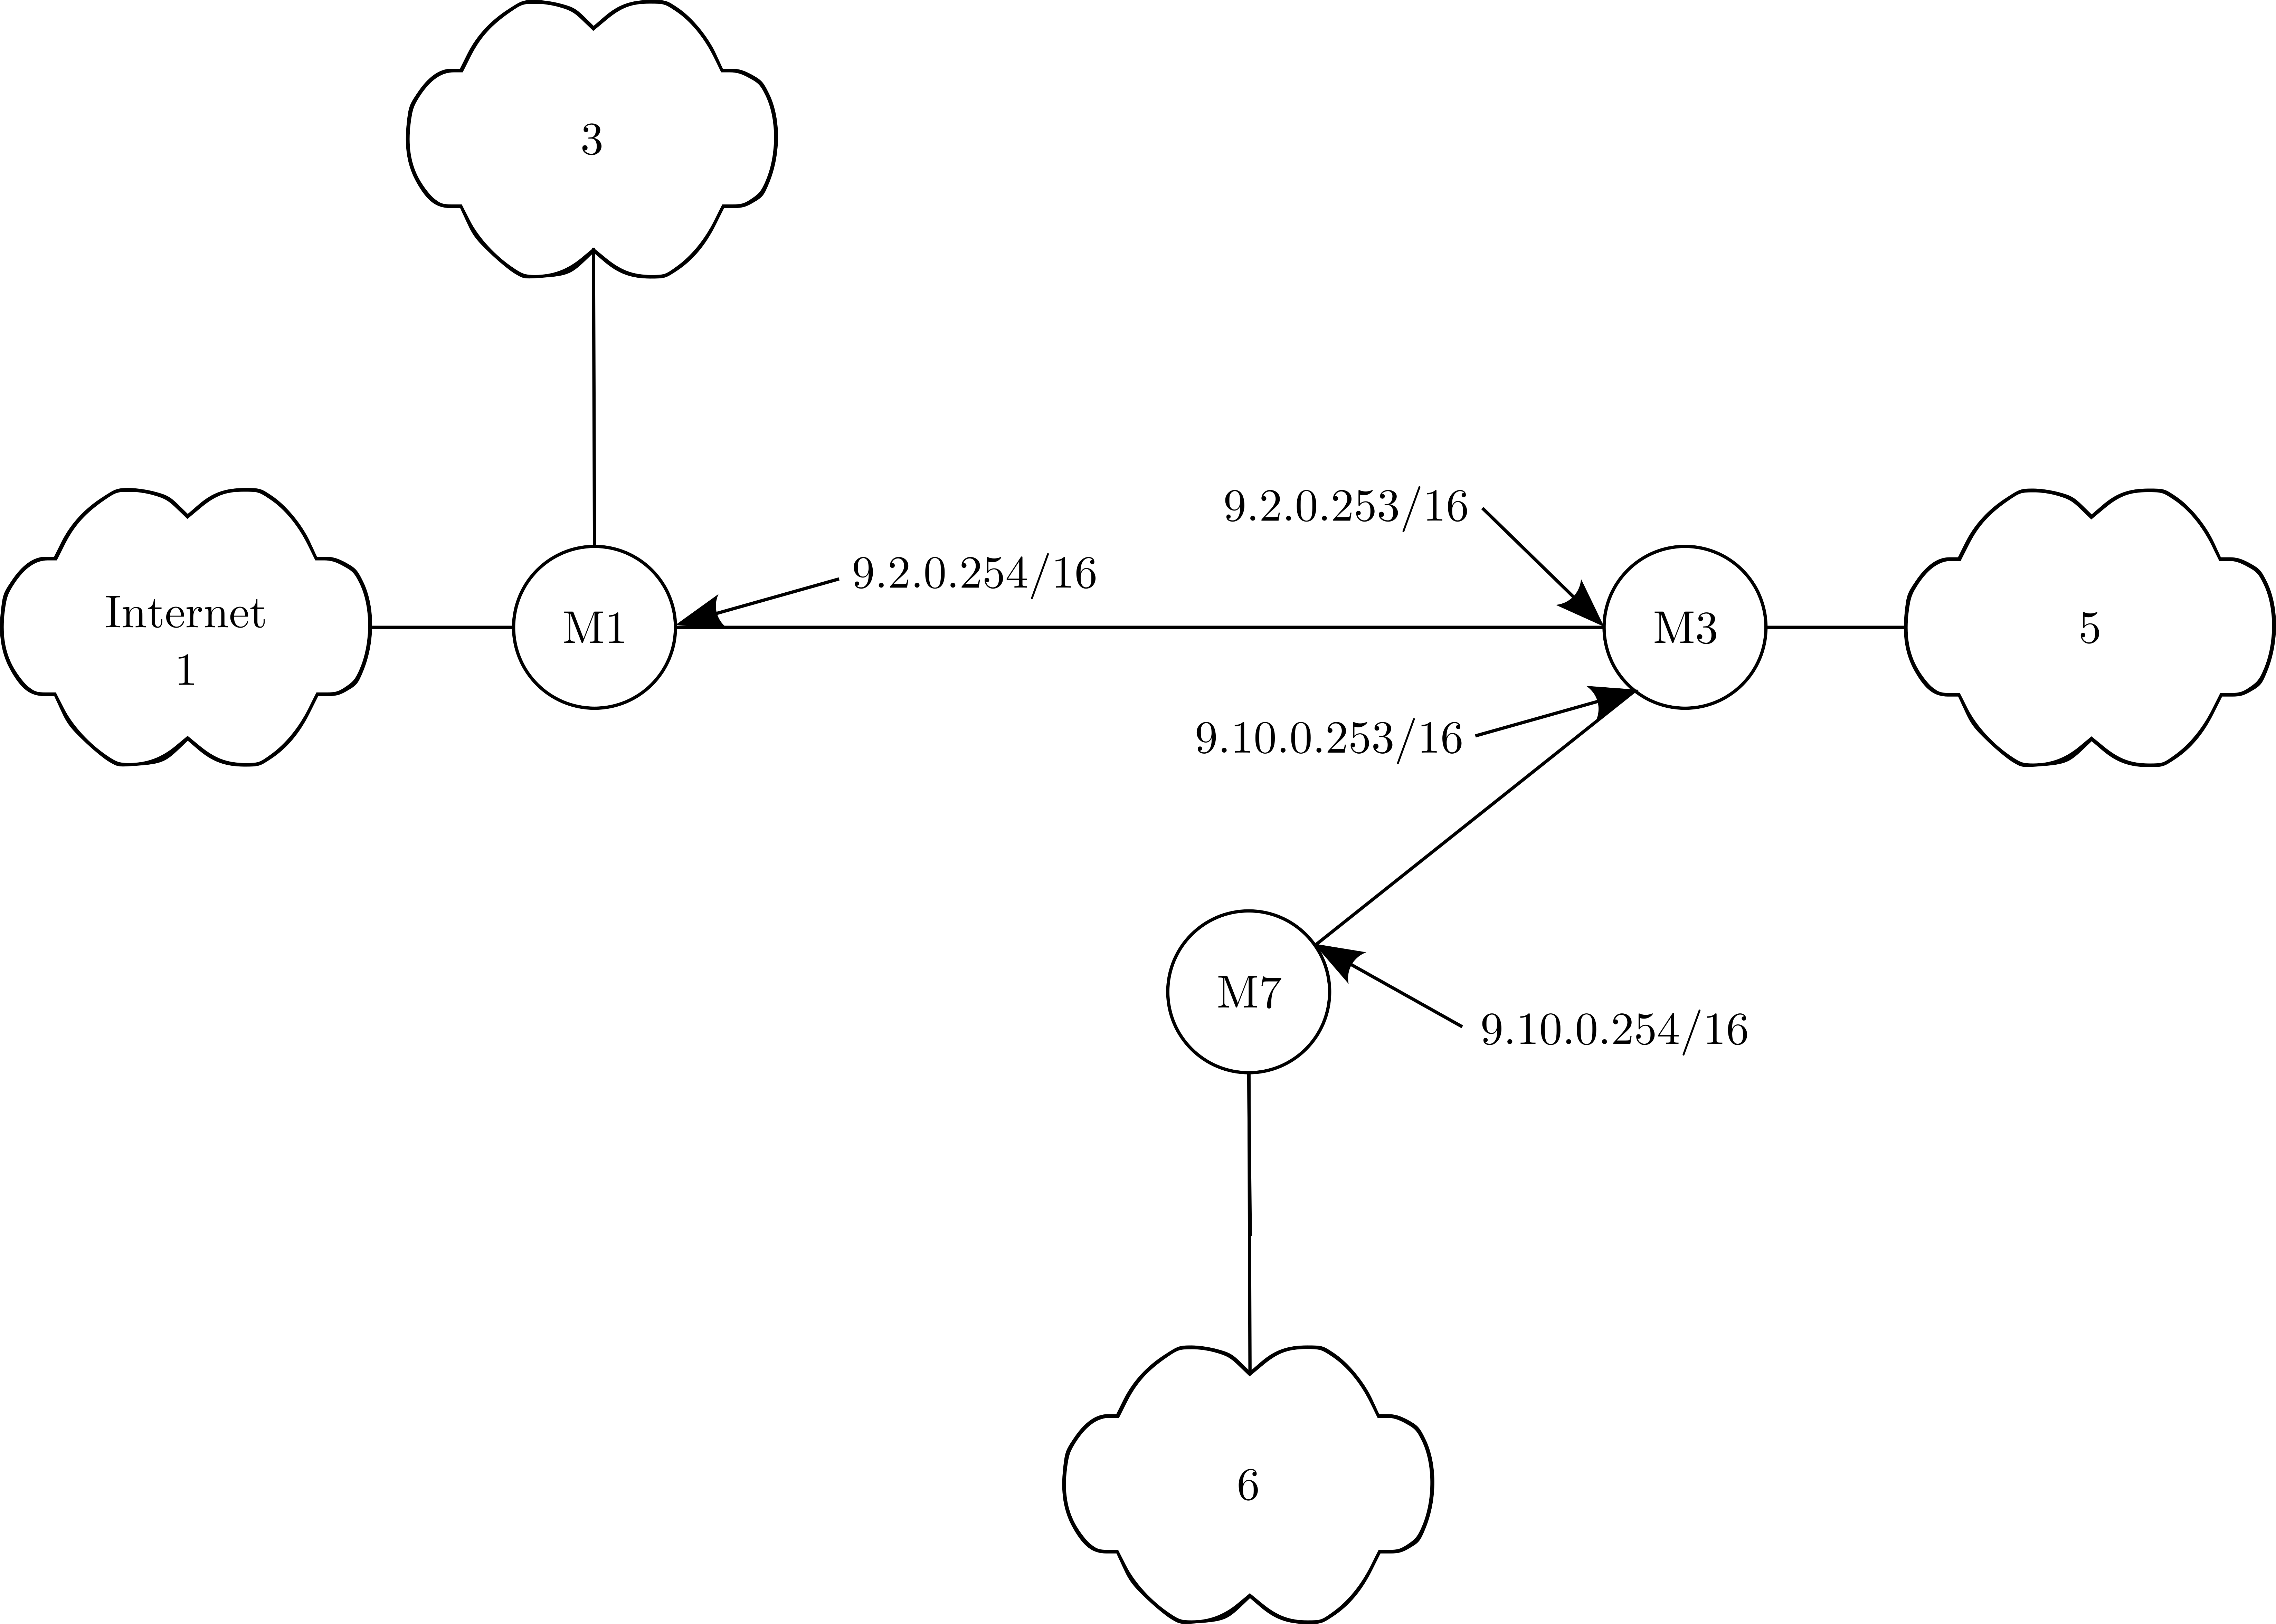
\includegraphics[width=0.8\textwidth]{images/network-scheme-1.png}
  \caption{Структура сети в соответствии с заданием}
  \label{fig:network-scheme-1}
\end{figure}

\subsection{Разбивка сетей}

Выполним разбивку сетей. По условию сеть 3 --- это сеть вида 192.168.32.0/19.
Определим минимально возможное количество разрядов в маске, которого достаточно
для получения 5 подсетей. Количество разрядов в маске, необходимых для
кодирования 5 подсетей, можно определить по формуле
\[
  N = \lceil \log_2 (K + 1) \rceil,
\]
где \(K\) --- количество подсетей. Для сети 3 количество разрядов равно
\[
  N = \log_2 (5 + 1) = 3.
\]
Длина маски, заданной по варианту: 11111111.11111111.11100000.0000000 --- 19
единиц. Так как к ним добавляются еще три разряда, кодирующих подсеть, то длина
маски составит 19 + 3 = 22 единицы.

Определим адреса подсетей и маски. Закодируем подсети в двоичной системе:
\begin{itemize}
  \item \textbf{подсеть 1}: 001;
  \item \textbf{подсеть 2}: 010;
  \item \textbf{подсеть 3}: 011;
  \item \textbf{подсеть 4}: 100;
  \item \textbf{подсеть 5}: 101.
\end{itemize}

Запишем адреса подсетей:
\begin{itemize}
  \item \textbf{подсеть 1}: 11000000.10101000.001\textbf{001}00.00000000 \qquad
  192.168.36.0;
  \item \textbf{подсеть 2}: 11000000.10101000.001\textbf{010}00.00000000 \qquad
  192.168.40.0;
  \item \textbf{подсеть 3}: 11000000.10101000.001\textbf{011}00.00000000 \qquad
  192.168.44.0;
  \item \textbf{подсеть 4}: 11000000.10101000.001\textbf{100}00.00000000 \qquad
  192.168.48.0;
  \item \textbf{подсеть 5}: 11000000.10101000.001\textbf{101}00.00000000 \qquad
  192.168.52.0.
\end{itemize}

Учитывая, что маска имеет длину 22 единицы, запишем ее:

\begin{quotation}
  11111111.11111111.11111100.0000000 \qquad 255.255.252.0
\end{quotation}

На примере подсети 1 определим широковещательный адрес, максимально возможное
количество узлов и диапазон адресов.

Широковещательный адрес определяется как побитовое логическое ИЛИ между
IP-адресом и инверсией маски:

\begin{quotation}
  11000000.10101000.00100100.00000000 \qquad 192.168.36.0

  \qquad \qquad \qquad \qquad |

  00000000.00000000.00000011.11111111 \qquad \; 0.0.3.255

  \qquad \qquad \qquad \qquad =

  11000000.10101000.00100111.11111111 \qquad \; 192.168.39.255
\end{quotation}

Максимально возможное количество узлов определяется количеством разрядов,
отведенных под номер узла. В нашем случае длина маски 22 разряда, тогда под узел
остается \(32 - 22 = 10\) разрядов. Тогда максимально возможно количество узлов
\(2^{10} - 2 = 1022\) узла. В этом случае диапазон выглядит следующим образом:
192.168.36.1 – 192.168.39.254.

Аналогично выполним разбивку других сетей. В результате получим следующую схему
сети, изображенную на рис. \ref{fig:network-scheme-2}.

\begin{figure}[H]
  \centering
  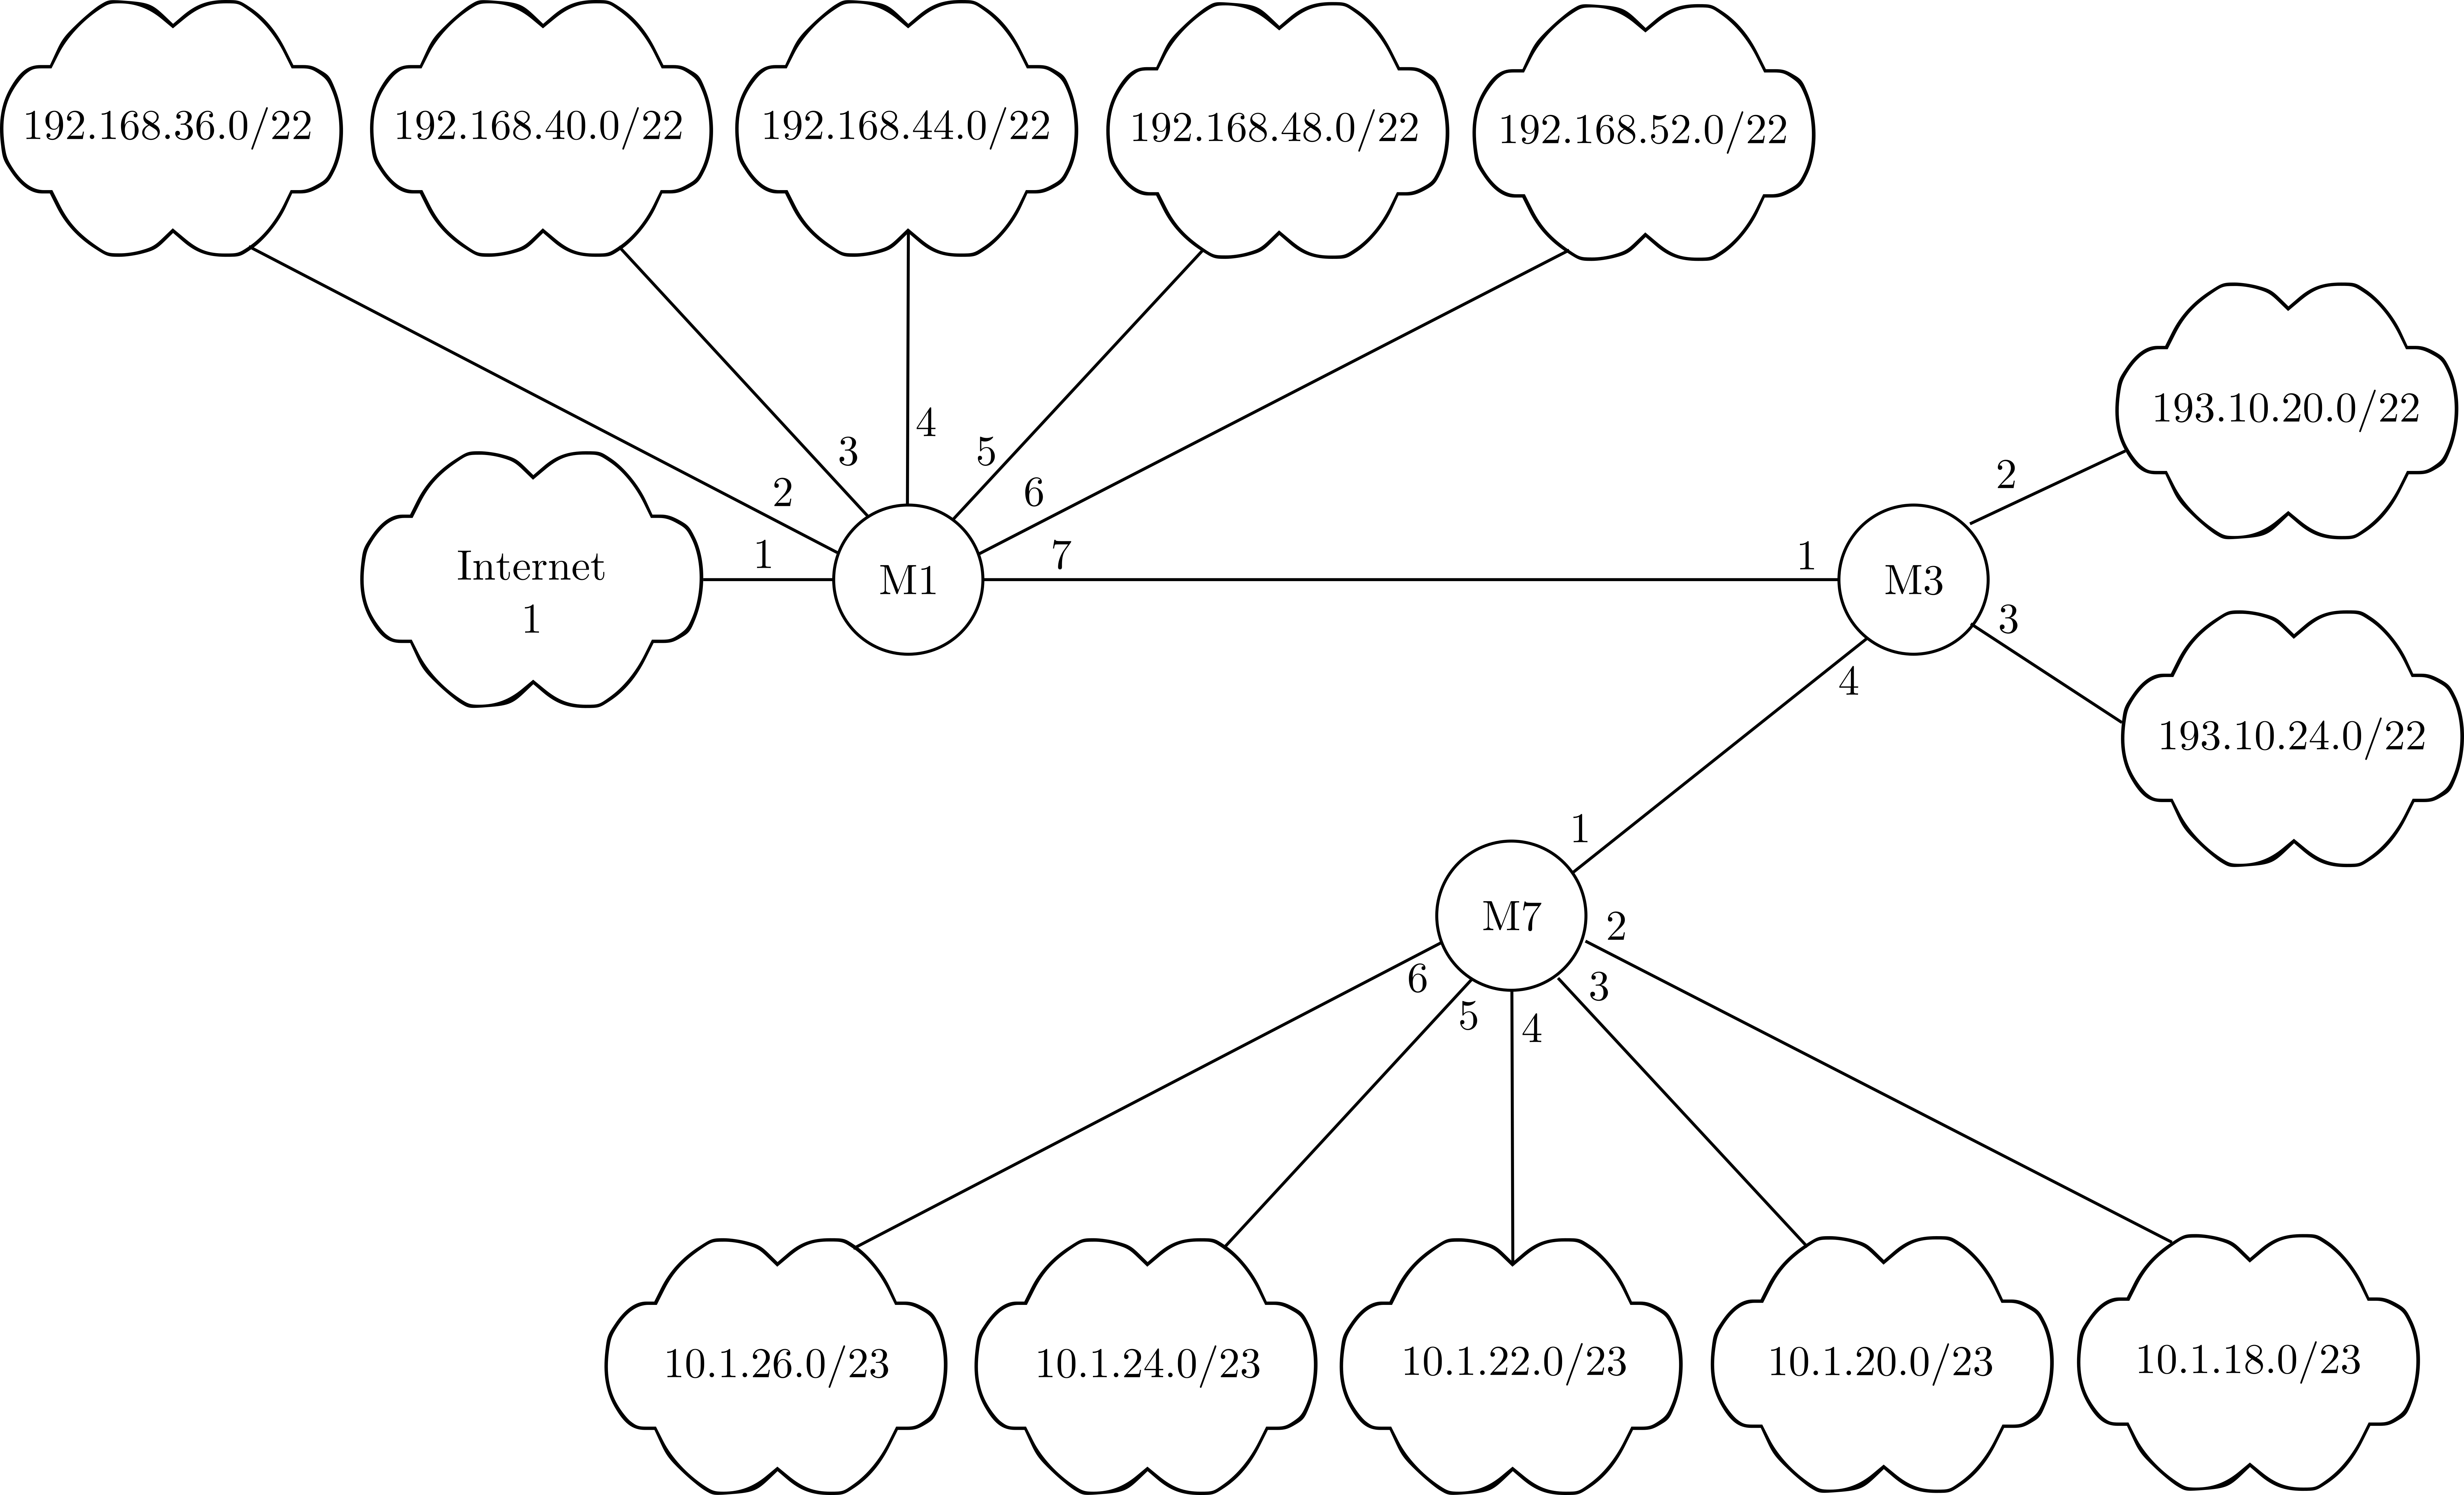
\includegraphics[width=0.8\textwidth]{images/network-scheme-2.png}
  \caption{Структура сети после разбивки}
  \label{fig:network-scheme-2}
\end{figure}

\subsection{Таблицы маршрутизации}

\begin{table}[H]
  \centering
  \setlength{\tabcolsep}{20pt}
  \caption{Адреса интерфейсов маршрутизаторов}
  \begin{tabular}{|c|c|c|}
    \hline
    Маршрутизатор      & Номер интерфейса & IP-адрес          \\
    \hline
    \multirow{7}{*}{1} & 1                & 194.44.183.17/28  \\
    \cline{2-3}
                       & 2                & 192.168.36.254/22 \\
    \cline{2-3}
                       & 3                & 192.168.40.254/22 \\
    \cline{2-3}
                       & 4                & 192.168.44.254/22 \\
    \cline{2-3}
                       & 5                & 192.168.48.254/22 \\
    \cline{2-3}
                       & 6                & 192.168.52.254/22 \\
    \cline{2-3}
                       & 7                & 9.2.0.254/16      \\
    \hline
    \multirow{4}{*}{3} & 1                & 9.2.0.253/16      \\
    \cline{2-3}
                       & 2                & 193.10.20.254/22  \\
    \cline{2-3}
                       & 3                & 193.10.24.254/22  \\
    \cline{2-3}
                       & 4                & 9.10.0.253/16     \\
    \hline
    \multirow{6}{*}{7} & 1                & 9.10.0.254/16     \\
    \cline{2-3}
                       & 2                & 10.1.18.254/23    \\
    \cline{2-3}
                       & 3                & 10.1.20.254/23    \\
    \cline{2-3}
                       & 4                & 10.1.22.254/23    \\
    \cline{2-3}
                       & 5                & 10.1.24.254/23    \\
    \cline{2-3}
                       & 6                & 10.1.26.254/23    \\
    \hline
  \end{tabular}
\end{table}

\begin{table}[H]
  \centering
  \setlength{\tabcolsep}{14pt}
  \caption{Таблица маршрутизации маршрутизатора М1}
  \begin{tabular}{|c|c|c|c|}
    \hline
    Адрес сети    & Маска сети      & Адрес шлюза   & Номер интерфейса \\
    \hline
    194.44.183.17 & 255.255.255.240 & 0.0.0.0       & 1                \\
    \hline
    192.168.36.0  & 255.255.252.0   & 0.0.0.0       & 2                \\
    \hline
    192.168.40.0  & 255.255.252.0   & 0.0.0.0       & 3                \\
    \hline
    192.168.44.0  & 255.255.252.0   & 0.0.0.0       & 4                \\
    \hline
    192.168.48.0  & 255.255.252.0   & 0.0.0.0       & 5                \\
    \hline
    192.168.52.0  & 255.255.252.0   & 0.0.0.0       & 6                \\
    \hline
    9.2.0.0       & 255.255.0.0     & 0.0.0.0       & 7                \\
    \hline
    193.10.16.0   & 255.255.240.0   & 9.2.0.253     & 7                \\
    \hline
    10.1.16.0     & 255.255.240.0   & 9.2.0.253     & 7                \\
    \hline
    0.0.0.0       & 0.0.0.0         & 194.44.183.17 & 1                \\
    \hline
  \end{tabular}
\end{table}

\begin{table}[H]
  \centering
  \setlength{\tabcolsep}{20pt}
  \caption{Таблица маршрутизации маршрутизатора М3}
  \begin{tabular}{|c|c|c|c|}
    \hline
    Адрес сети   & Маска сети    & Адрес шлюза & Номер интерфейса \\
    \hline
    192.168.32.0 & 255.255.224.0 & 9.2.0.254   & 1                \\
    \hline
    9.2.0.0      & 255.255.0.0   & 0.0.0.0     & 1                \\
    \hline
    193.10.20.0  & 255.255.252.0 & 0.0.0.0     & 2                \\
    \hline
    193.10.24.0  & 255.255.252.0 & 0.0.0.0     & 3                \\
    \hline
    10.1.16.0    & 255.255.240.0 & 9.10.0.254  & 4                \\
    \hline
    9.10.0.0     & 255.255.0.0   & 0.0.0.0     & 4                \\
    \hline
    0.0.0.0      & 0.0.0.0       & 9.2.0.254   & 1                \\
    \hline
  \end{tabular}
\end{table}

\begin{table}[H]
  \centering
  \setlength{\tabcolsep}{20pt}
  \caption{Таблица маршрутизации маршрутизатора М7}
  \begin{tabular}{|c|c|c|c|}
    \hline
    Адрес сети   & Маска сети    & Адрес шлюза & Номер интерфейса \\
    \hline
    192.168.32.0 & 255.255.224.0 & 9.10.0.253  & 1                \\
    \hline
    193.10.16.0  & 255.255.240.0 & 9.10.0.253  & 1                \\
    \hline
    9.10.0.0     & 255.255.0.0   & 0.0.0.0     & 1                \\
    \hline
    10.1.18.0    & 255.255.254.0 & 0.0.0.0     & 2                \\
    \hline
    10.1.20.0    & 255.255.254.0 & 0.0.0.0     & 3                \\
    \hline
    10.1.22.0    & 255.255.254.0 & 0.0.0.0     & 4                \\
    \hline
    10.1.24.0    & 255.255.254.0 & 0.0.0.0     & 5                \\
    \hline
    10.1.26.0    & 255.255.254.0 & 0.0.0.0     & 6                \\
    \hline
    0.0.0.0      & 0.0.0.0       & 9.10.0.253  & 1                \\
    \hline
  \end{tabular}
\end{table}

\section{Моделирование сети в Cisco Packet Tracer}

\subsection{Настройка маршрутизаторов}

В качестве маршрутизаторов были использованы маршрутизаторы типа
Router-PT-Empty. По заданию сеть состоит из трех маршрутизаторов. После их
добавления получим сеть, изображенную на рис. \ref{fig:network-1.png}.

\begin{figure}[H]
  \centering
  \fbox{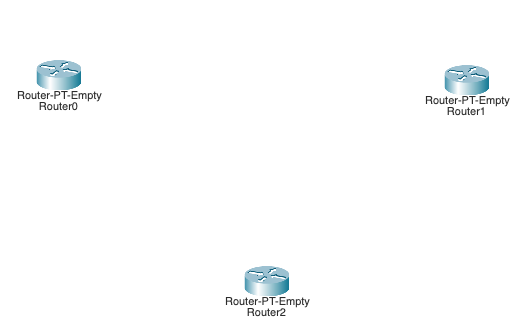
\includegraphics[width=0.6\textwidth]{images/network/1.png}}
  \caption{Логическое представление сети}
  \label{fig:network-1.png}
\end{figure}

В физической конфигурации каждого маршрутизатора было добавлено необходимое
количество модулей типа PT-ROUTER-NM-1CFE (рис. \ref{fig:network-2.png}). Так
для маршрутизатора M1 было добавлено 6 модулей, для маршрутизатора M3 — 4
модуля, для маршрутизатора M7 — 6 модулей.

\begin{figure}[H]
  \centering
  \fbox{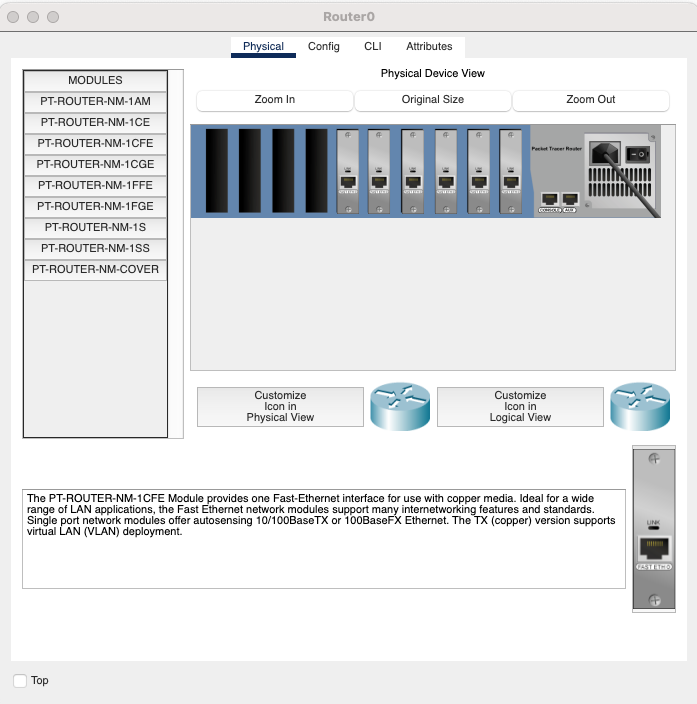
\includegraphics[width=0.6\textwidth]{images/network/2.png}}
  \caption{Физическая конфигурация маршрутизатора M1}
  \label{fig:network-2.png}
\end{figure}

Также каждый маршрутизатор был настроен с помощью командной строки. Для
включения и перехода в режим конфигурации были использованы следующие команды:
\begin{minted}{text}
  enable
  config t
\end{minted}
Затем для у маршрутизатора для каждого из портов были указаны соответствующие
IP-адреса. В качестве примера приведены команды для настройки интерфейса
FastEthernet0/0 на маршрутизаторе M1:
\begin{minted}{text}
  int FastEthernet0/0
  ip address 192.168.36.254 255.255.252.0
  no shut
\end{minted}
В итоге на маршрутизаторе M1 получилась конфигурация портов, изображенная на
рис. \ref{fig:int-brief/m1.png}. Аналогичные действия были проделаны на всех
маршрутизаторах. Для получения информации о конфигурации портов использовалась
команда \texttt{ip int brief}.

\begin{figure}[H]
  \centering
  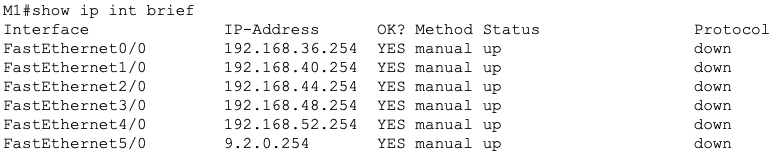
\includegraphics[width=0.7\textwidth]{images/int-brief/m1.png}
  \caption{Описание интерфейсов маршрутизатора M1}
  \label{fig:int-brief/m1.png}
\end{figure}

\subsection{Настройка рабочих станций}

После добавления маршрутизаторов в сеть были добавлены рабочие станции (рис.
\ref{fig:network-4.png}). Для каждой рабочей станции были настроены IP-адрес,
маска подсети, а также IP-адрес шлюза по умолчанию. На рис.
\ref{fig:network-5.png} представлен пример настройки устройства PC-PT PC0.

\begin{figure}[H]
  \centering
  \fbox{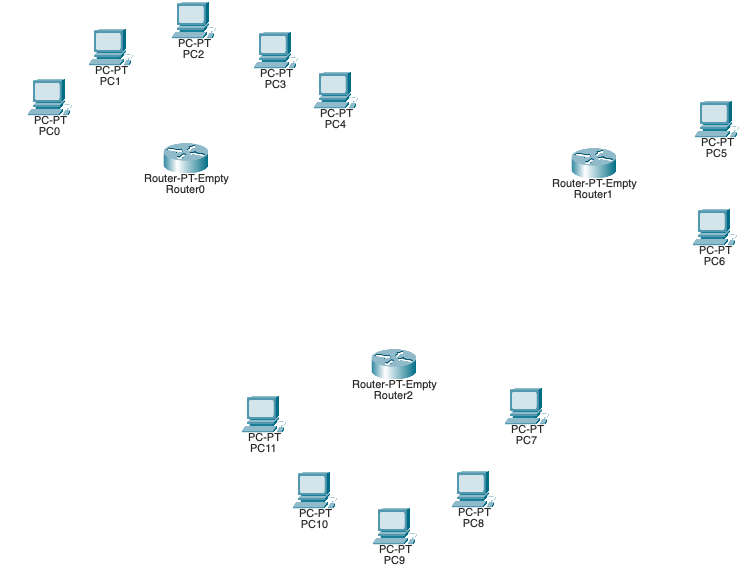
\includegraphics[width=0.7\textwidth]{images/network/4.png}}
  \caption{Логическое представление сети}
  \label{fig:network-4.png}
\end{figure}

\begin{figure}[H]
  \centering
  \fbox{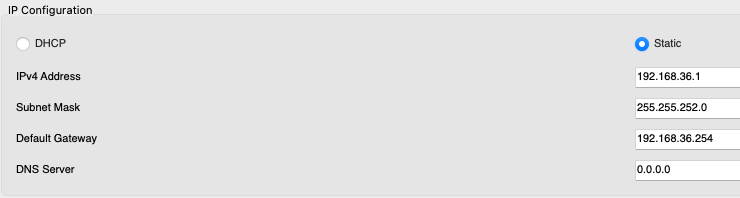
\includegraphics[width=0.7\textwidth]{images/network/5.png}}
  \caption{Настройка рабочей станции}
  \label{fig:network-5.png}
\end{figure}

\subsection{Соединение устройств между собой}

После добавления всех необходимых устройств, согласно схеме
\ref{fig:network-scheme-2}, все рабочие станции были соединены со своими
маршрутизаторами, а маршрутизаторы --- между собой. В итоге получилась схема,
изображенная на рис. \ref{fig:network-6.png}. В качестве кабеля был использован
кабель под названием Cross-Over.

\begin{figure}[H]
  \centering
  \fbox{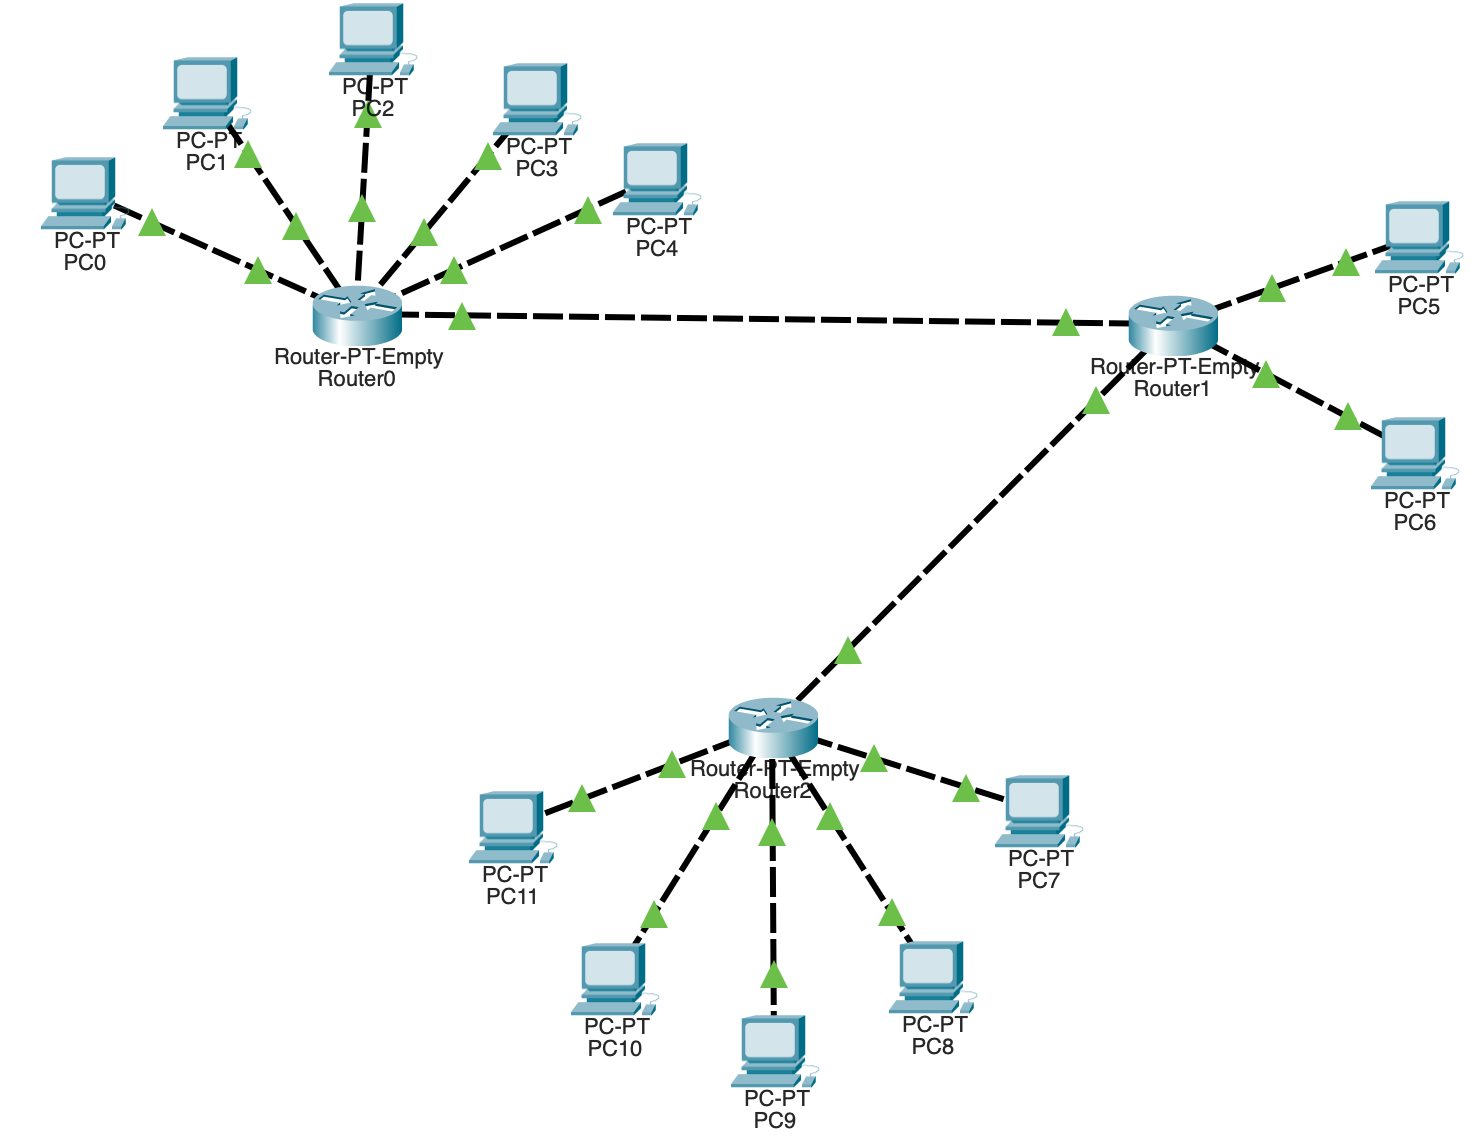
\includegraphics[width=0.7\textwidth]{images/network/6.png}}
  \caption{Логическое представление сети}
  \label{fig:network-6.png}
\end{figure}

Для проверки соединения были выбраны рабочие станции PC-PT PC0 с IP-адресом
192.168.36.1 и PC-PT PC11 с IP-адресом 10.1.26.1. На рис.
\ref{fig:ping/before.png} показан результат выполнения команды \texttt{ping} на
рабочей станции PC0, которая проверяет доступность PC11. В итоге, ни один из
пакетов не смог дойти до адресата.

\begin{figure}[H]
  \centering
  \fbox{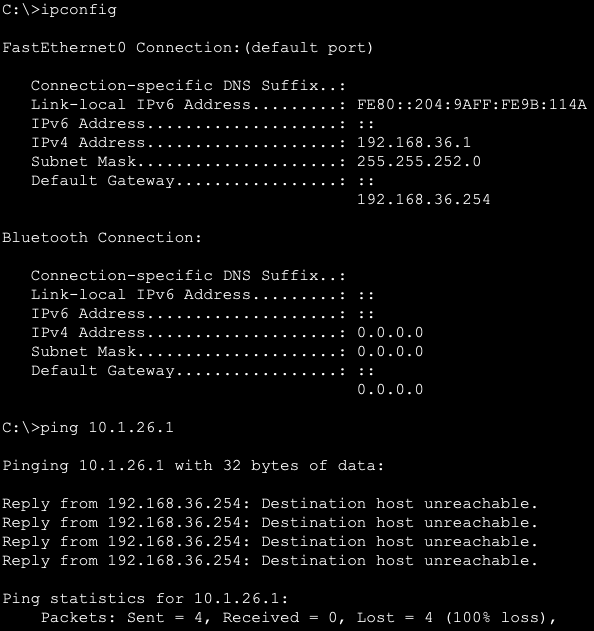
\includegraphics[width=0.6\textwidth]{images/ping/before.png}}
  \caption{Результат проверки доступности}
  \label{fig:ping/before.png}
\end{figure}

Это произошло из-за того, что у маршрутизаторов не заполнены таблицы
маршрутизации.

\subsection{Настройка таблицы маршрутизации}

Чтобы исправить проблему, описанную выше, необходимо на каждом маршрутизаторе
прописать маршруты с помощью команды \texttt{ip route}. В качестве примера
представлены команды для маршрутизатора M1:
\begin{minted}{text}
  ip route 193.10.16.0 255.255.240.0 9.2.0.253
  ip route 10.1.16.0 255.255.240.0 9.2.0.253
  ip route 0.0.0.0 0.0.0.0 9.2.0.253
\end{minted}
После добавления этих маршрутов, на маршрутизаторе M1 получилась таблица
маршрутизации, изображенная на рис. \ref{fig:ip-route/m1-after.png}. Для
получения информации о маршрутах использовалась команда \texttt{show ip route}.

\begin{figure}[H]
  \centering
  \fbox{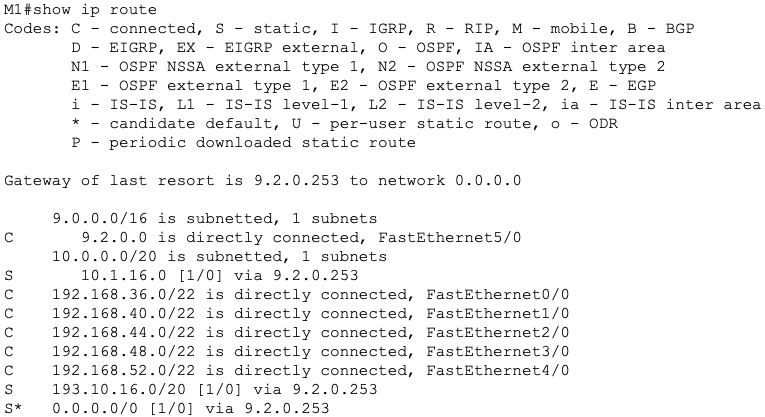
\includegraphics[width=0.6\textwidth]{images/ip-route/m1-after.png}}
  \caption{Таблица маршрутизации M1}
  \label{fig:ip-route/m1-after.png}
\end{figure}

Теперь при проверке доступности с рабочей станции PC-PT PC0 с IP-адресом
192.168.36.1 другой рабочей станции PC-PT PC11 с IP-адресом 10.1.26.1 пакеты
успешно доходят до адресата (рис. \ref{fig:ping/after.png}).

\begin{figure}[H]
  \centering
  \fbox{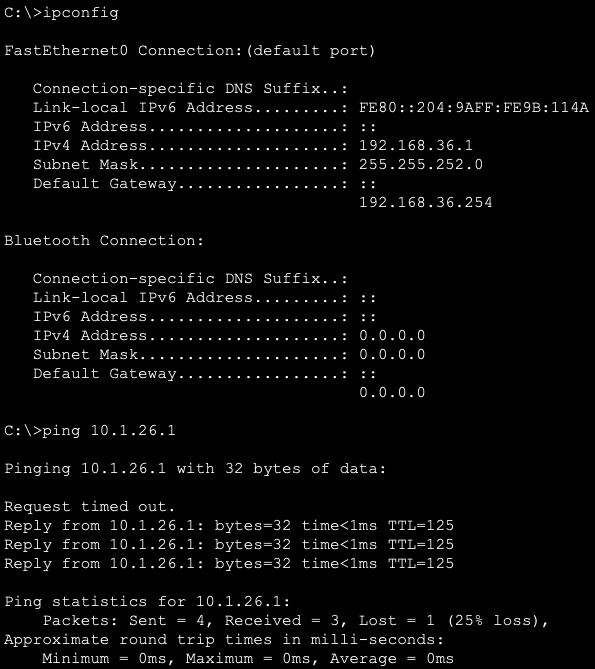
\includegraphics[width=0.6\textwidth]{images/ping/after.png}}
  \caption{Результат проверки доступности}
  \label{fig:ping/after.png}
\end{figure}

\subsection{Визуализация работы сети}

Для визуализации работы сети был использован режим <<Simulation mode>>. С
помощью кнопки <<Add simple PDU>> был создан простой PDU. В качестве устройств
снова были выбраны рабочие станции PC-PT PC0 и PC-PT P11. Отправителем был
назначен PC0 (рис. \ref{fig:visualization/reachable/start.png}), а получателем
--- PC11. После запуска симуляции пакет был успешно доставлен до адресата (рис.
\ref{fig:visualization/reachable/end.png}).

\begin{figure}[H]
  \centering
  \fbox{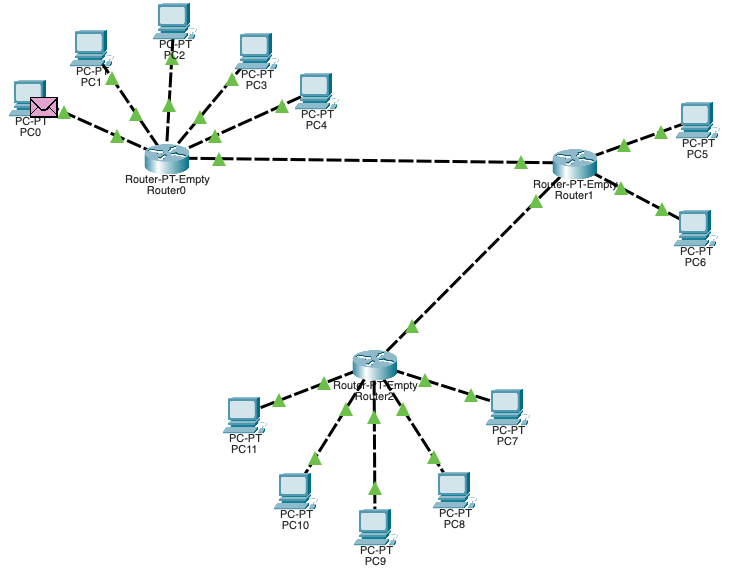
\includegraphics[width=0.7\textwidth]{images/visualization/reachable/start.png}}
  \caption{Отправление пакета в режиме симуляции}
  \label{fig:visualization/reachable/start.png}
\end{figure}

\begin{figure}[H]
  \centering
  \fbox{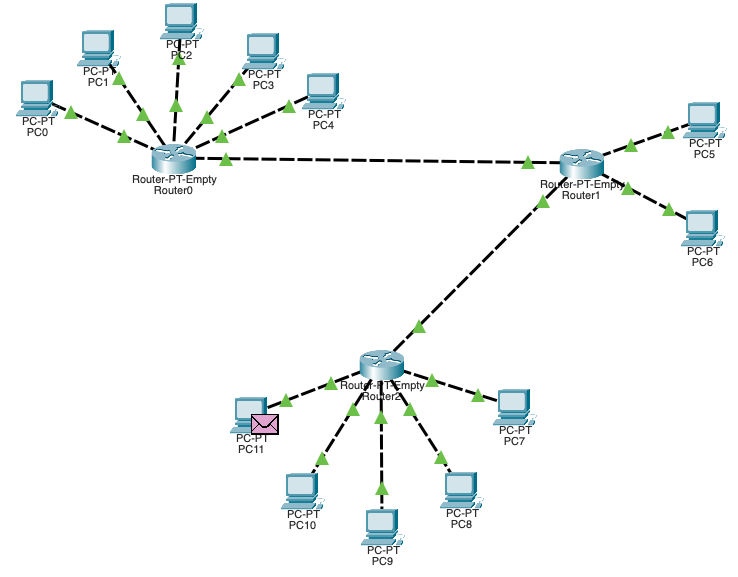
\includegraphics[width=0.7\textwidth]{images/visualization/reachable/end.png}}
  \caption{Успешное получение пакета в режиме симуляции}
  \label{fig:visualization/reachable/end.png}
\end{figure}

В случае, если маршруты будут удалены из, например, маршрутизатора M2, как
показано на рис. \ref{fig:visualization/unreachable/remove.png}, то пакет не
будет доставлен, поскольку маршрутизатор M2 не знает, куда отправлять данный
пакет дальше (рис. \ref{fig:visualization/unreachable/end.png}).

\begin{figure}[H]
  \centering
  \fbox{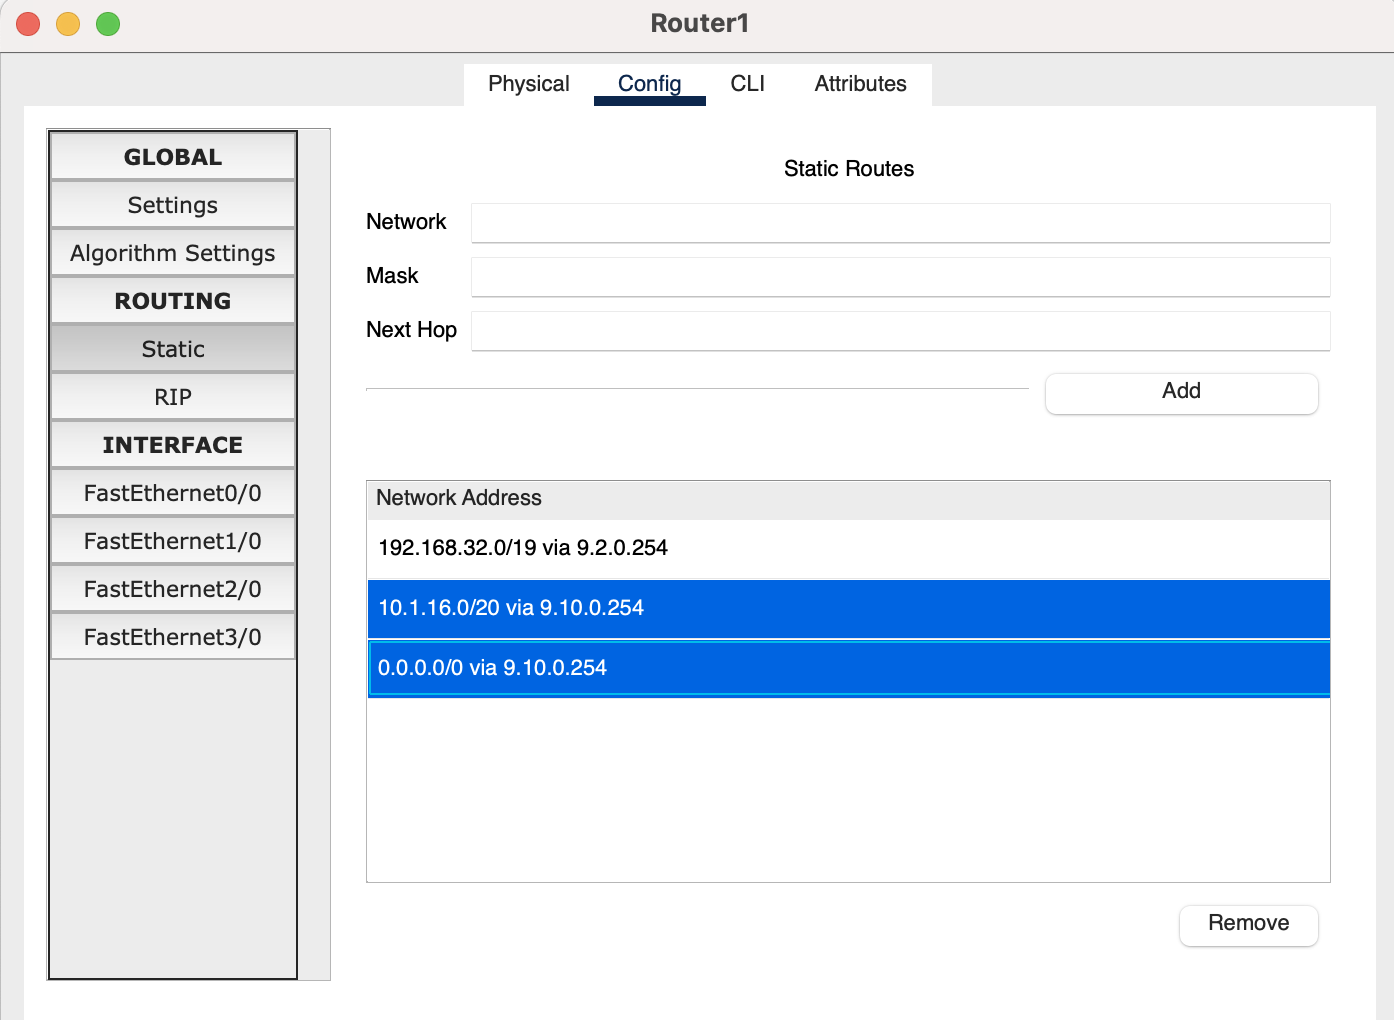
\includegraphics[width=0.6\textwidth]{images/visualization/unreachable/remove.png}}
  \caption{Удаление маршрутов из таблицы маршрутизации}
  \label{fig:visualization/unreachable/remove.png}
\end{figure}

\begin{figure}[H]
  \centering
  \fbox{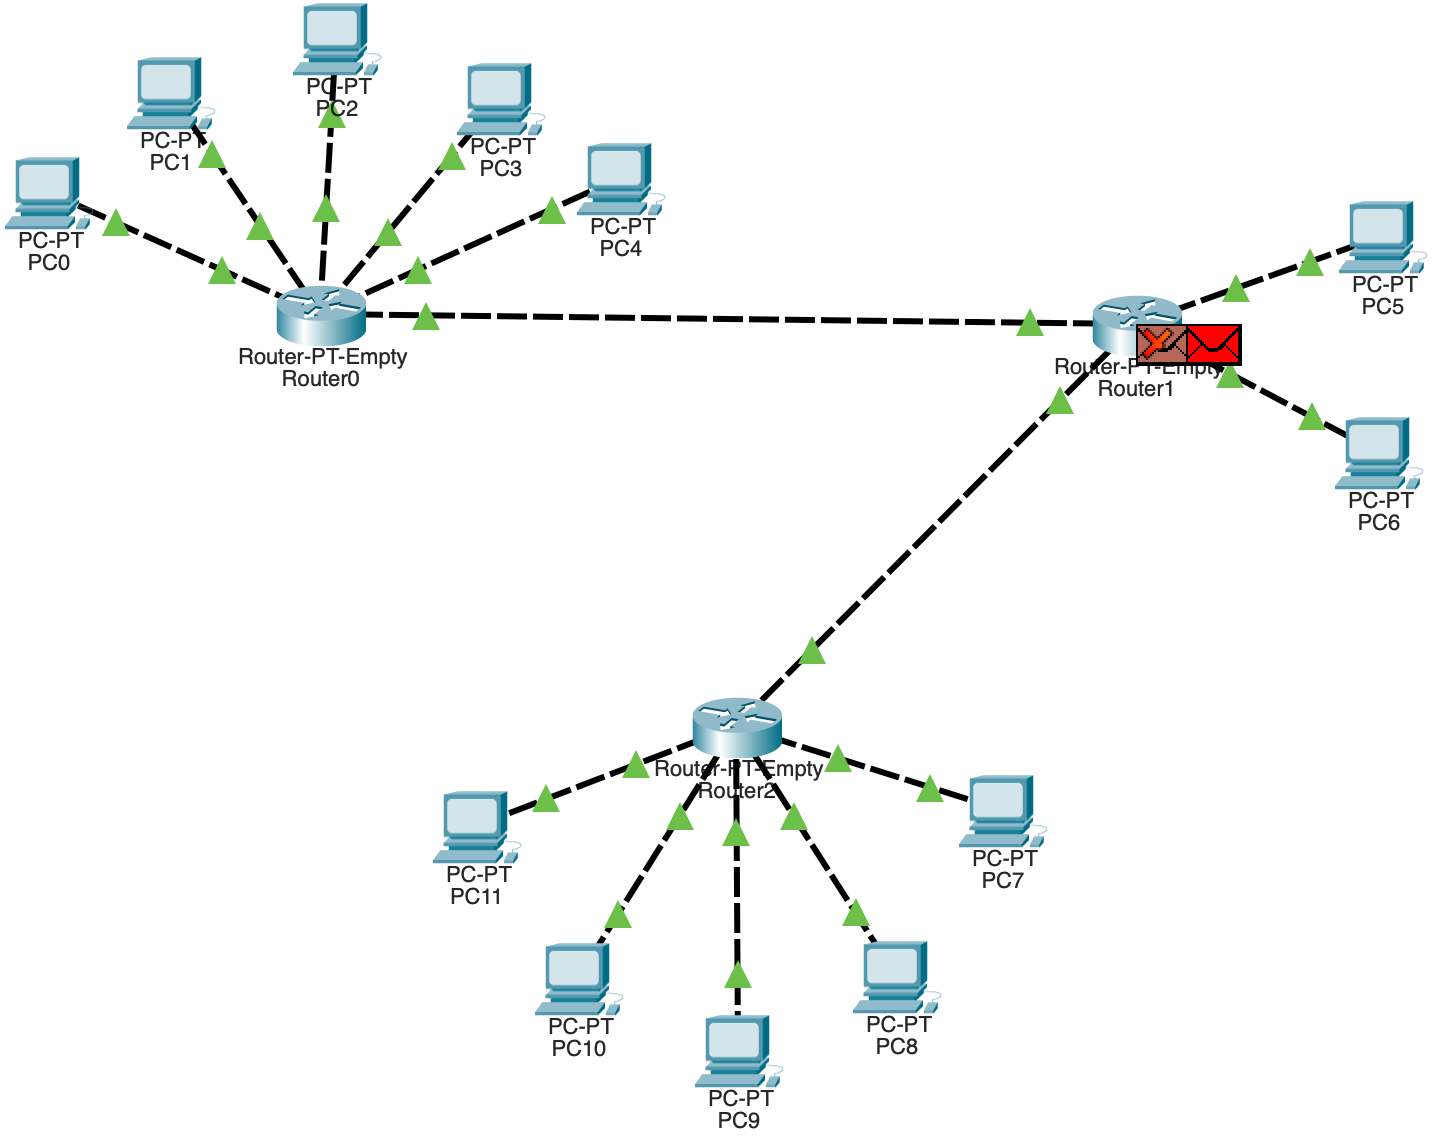
\includegraphics[width=0.7\textwidth]{images/visualization/unreachable/end.png}}
  \caption{Безуспешная попытка получения пакета}
  \label{fig:visualization/unreachable/end.png}
\end{figure}

\section{Заключение}

В ходе выполнения лабораторной работы я изучил основные принципы IP адресации,
получил практические навыки в построении сетей и подсетей разных классов с
использованием современных возможностей протокола IP, изучил базовые принципы
маршрутизации в IP-сетях, а также научился конфигурировать сетевое оборудование
с помощью симулятора CISCO PacketTracer.

\end{document}
